\section{table2}
\hspace{-1cm}
	\centering
	\begin{tabular}{p{4cm}p{10cm}}
		\hline
		Title & tourism app \\
		\hline
		Date & 16th April 2019 \\
		\hline
		Scene & 3 of 4 \\
		\hline
		Description & The selected page \\
		\hline
		Links From Scenes & Scene 1, Scene 2 \\
		\hline
		Links To Scenes & Scene 1, Scene 2 \\
		\hline
		\multicolumn{2}{c}{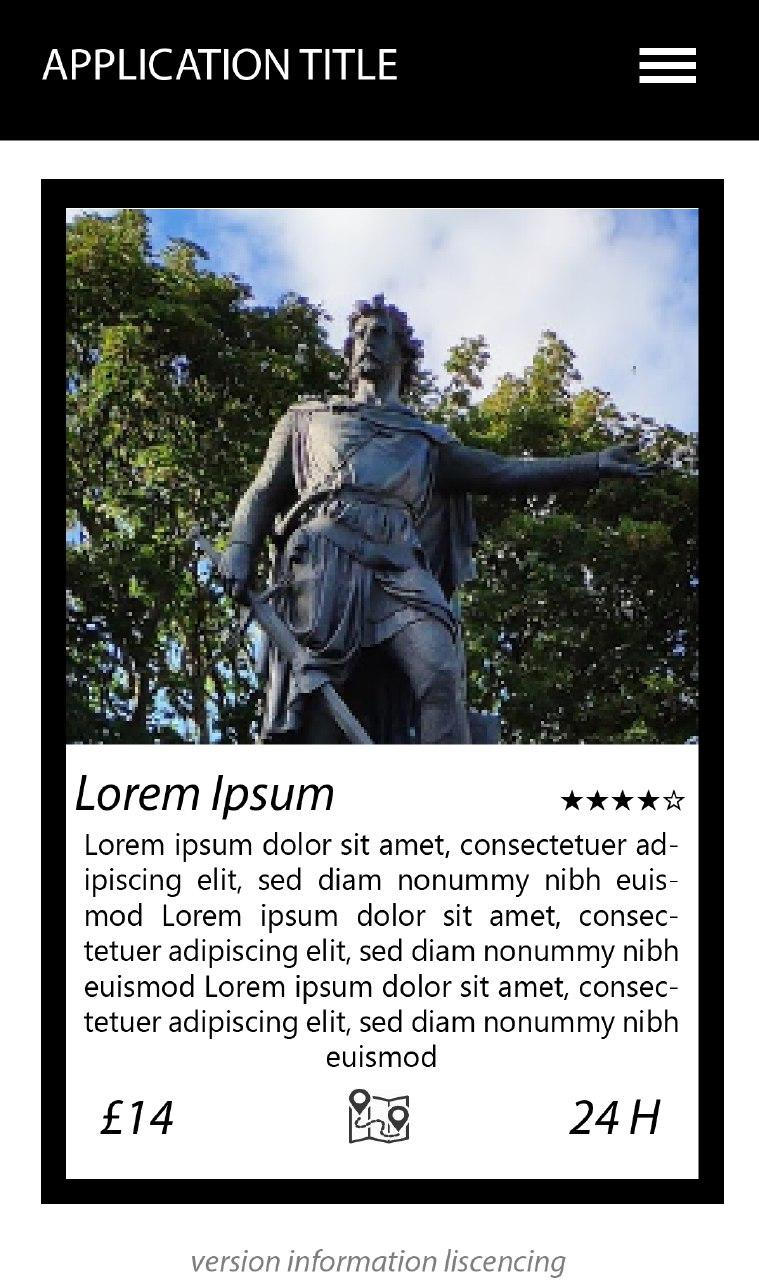
\includegraphics[width=0.5\linewidth]{images/screen2.jpg}} \\
		\hline
		Background & Solid white background on black to highlight the "card design" \\
		\hline
		Colour Scehemes Used & Default to black and white but would import from the system theme so users feel immersed \\
		\hline
		Text Attributes & Again, follows system theme (usually a sans-serif font). \\
		\hline
		Audio Files & N/A \\
		\hline
		Video Files & N/A \\
		\hline
		Stills Files & Header Image for the Location \\
		\hline
		Animations / Movie Clips & N/A \\
		\hline
		\multicolumn{2}{c}{Interface Components (buttons, widgets)} \\
		\hline
		\multicolumn{2}{p{14cm}}{This page contains all of the relevant information pertaining to the attraction. The main content is the image of the location selected by either votes of users or by the maintainers of the attraction. Following this is the Title and the rating on the same line. The rating is powered by user feedback. Next is the description of the attraction of the site which again is chosen by the maintainers. Finally on at the bottom is the price of the venue, a link to get directions to the site and the opening hours.} \\
		\hline
	\end{tabular}
